\section{A finite Gaussian and residual construction across all three applications}
\label{sec:triad-bridge}

The construction of \Cref{sec:gaussian-bridge} extends to a third
object, the assignment space of a CNF formula.  Let \(\varphi\) be a CNF
formula in \(n\) Boolean variables, let \(A_{n}=\{0,1\}^{n}\), and let
\(s_{\varphi}:A_{n}\to\{0,1\}\) be its assignment verifier,
\(s_{\varphi}(w)=1\) exactly when \(w\) satisfies \(\varphi\).  The
satisfiability language \(L_{\mathrm{SAT}}\) is taken in the bitstring
encoding of CNF formulas used for the machine-defined classes \(P\),
\(NP\) and \(FP\) in the P-versus-NP companion \cite{Tsiokos2026PvNP};
the verifier agrees with that encoding, in the sense that the encoding
of \(\varphi\) lies in \(L_{\mathrm{SAT}}\) exactly when some \(w\)
satisfies \(\varphi\).  We regard \(s_{\varphi}\) as a vector in the
\(2^{n}\)-dimensional Euclidean space \(\mathbb R^{A_{n}}\).

\subsection{The shared kernel and the SAT residual}

The finite form of the construction sums the heat observation
\(N_{a,b}\) of \eqref{eq:joint-heat-kernel} over a finite weighted set
of points.  On a reflected zero window the points are the spectral
coordinates of the zeros, with their weights.  On \(A_{n}\) the weight
of \(w\) is \(s_{\varphi}(w)\) and the point is
\(\frac12+i\operatorname{code}(w)\), where \(\operatorname{code}(w)\)
is the natural number with binary digits \(w\); its spectral coordinate
is the real number \(\operatorname{code}(w)\).  This choice of points is
a convention.  For real \(\kappa\) the resulting mass is
\begin{equation}
\label{eq:triad-sat-mass}
 M_\kappa(\varphi)=\sum_{w\in A_n}s_\varphi(w)\,
       e^{-\kappa\operatorname{code}(w)^2}.
\end{equation}
Every term is nonnegative and the terms with \(s_{\varphi}(w)=1\) are
positive, so \(M_{\kappa}(\varphi)>0\) exactly when \(\varphi\) is
satisfiable.  The same holds for any \(\{0,1\}\)-valued filter in place
of \(s_{\varphi}\); what is specific to SAT is the verifier, its
agreement with the encoded language, and the clause and branching laws
below.

Adding a clause \(\chi\) removes exactly the assignments that satisfy
\(\varphi\) and fail \(\chi\):
\begin{equation}
\label{eq:triad-clause-residual}
 M_\kappa(\varphi\wedge\chi)
   =M_\kappa(\varphi)-
     \sum_{\substack{w\models\varphi\\w\not\models\chi}}
       e^{-\kappa\operatorname{code}(w)^2}.
\end{equation}

On the Navier--Stokes side we use a \emph{frame} of three mild
solutions.  Fix \(\gamma>5/2\) and \(\nu,t_{0}>0\), and for
\(i=1,2,3\) let \(g^{(i)}\) be the maximal mild solution, in the
weighted coordinates of \Cref{sec:gaussian-bridge}, with initial state
\(g^{(i)}_{0}(\xi)=e^{-4\pi^{2}\nu t_{0}|\xi|^{2}}P(\xi)e_{i}\), where
\(P(\xi)\) is the Leray projection symbol and \(e_{i}\) the \(i\)-th
coordinate vector; the physical initial amplitude is
\((1+|\xi|^{2})^{-\gamma/2}g^{(i)}_{0}(\xi)\), the transform of a real,
divergence-free field.  A time \(\tau\ge0\) is admissible for the frame
if it is admissible for all three data; a positive such time exists.
The \emph{frame trace} of the observation at \(\tau\) is
\(T_{a,z}(\tau)=\sum_{i}\bigl(\mathcal O_{a,\theta_{\rm axis},z}(g^{(i)}(\tau))\bigr)_{i}\),
and \(T^{\mathcal D}_{a,z}(\tau)\) is the same expression with the
Duhamel terms \(\mathcal D[g^{(i)}](\tau)\) in place of \(g^{(i)}(\tau)\).
Since the Leray symbol has trace \(2\), the mild equation gives
\[
  \tfrac12\bigl(T_{a,z}(\tau)+T^{\mathcal D}_{a,z}(\tau)\bigr)=N_{a,b}(z),
  \qquad b=4\pi^{2}\nu(\tau+t_{0}).
\]
We call the left-hand side the \emph{normalized frame value}.  Replacing
\(N_{a,b}\) by it in the definition of the logarithmic excess of
\Cref{sec:gaussian-bridge} gives the \emph{frame heat excess} of a
window, and, by the displayed identity, every heat-side identity
transfers to the frame with the Duhamel terms kept.  In particular
\eqref{eq:triad-clause-residual} holds with each term
\(e^{-\kappa\operatorname{code}(w)^{2}}\) replaced by the raw frame value
\(T_{a,z}+T^{\mathcal D}_{a,z}\) at \(z=\operatorname{code}(w)\), which is
\(2(\pi/(a+b))^{3/2}\) times that term.  These are exact identities,
not estimates of the nonlinear terms.

The common probe on a finite index set \(I\) is the sum of coordinates,
\(L_{I}(v)=\sum_{i\in I}v_{i}\), and the residual \(\Xi(L_{I})\) is the
orthogonal projection onto \(\ker L_{I}\); its complement
\(\Pi(L_{I})=1-\Xi(L_{I})\) is the projection onto the constant vectors,
the \emph{native} channel.  On a reflected zero window the probe of the
displacement vanishes, \(L_{W}(v_{W})=0\), so the displacement lies
entirely in the residual.  On the assignment space,
\(L_{A_{n}}(s_{\varphi})\) is the number of satisfying assignments,
which is positive exactly when the encoding of \(\varphi\) lies in
\(L_{\mathrm{SAT}}\).  Thus satisfiability is read in the native
channel.  The residual alone does not detect it: the residual of
\(s_{\varphi}\) vanishes both for the empty conjunction (every
assignment satisfies it) and for a formula containing the empty clause
(none does).

A unit clause \(x_{i}=\beta\) acts on states by the mask
\((M_{i,\beta}v)(w)=v(w)\) if \(w_{i}=\beta\) and \(0\) otherwise, so
that \(s_{\varphi\wedge(x_{i}=\beta)}=M_{i,\beta}s_{\varphi}\).  Since
\(\Xi=1-\Pi\), the commutator of the mask with the residual is
\[
  \Xi M_{i,\beta}s_{\varphi}-M_{i,\beta}\Xi s_{\varphi}
  =M_{i,\beta}\Pi s_{\varphi}-\Pi M_{i,\beta}s_{\varphi}.
\]
A one-variable example shows that the mask need not commute with
\(\Xi\).  No operation on zero windows is identified with the mask.

\begin{theorem}[Concrete Gaussian--residual triad]
\label{thm:concrete-triad-gaussian-xi}
Let \(\gamma>5/2\), \(\nu,t_{0}>0\) and \(a>0\), let \(\tau\ge0\) be
admissible for the frame, and put \(t=\tau+t_{0}\),
\(b=4\pi^{2}\nu t\) and \(\kappa=ab/(a+b)\).  Let \(W\) be a reflected
window with unit weights and \(\rho\in W\), and let \(\varphi\) be a CNF
formula in \(n\) variables, \(\chi\) a clause, \(i\le n\) and
\(\beta\in\{0,1\}\).  Then:
\begin{enumerate}
\item the frame heat excess of \(W\) equals
  \(\kappa\,\|\Xi(L_{W})v_{W}\|^{2}\), and \(L_{W}(v_{W})=0\);
\item the raw frame value \(T_{a,z}+T^{\mathcal D}_{a,z}\) summed over the
  satisfying assignments of \(\varphi\), at \(z=\operatorname{code}(w)\),
  is nonzero exactly when
  \(\|\Pi s_{\varphi}\|^{2}+\|\Xi s_{\varphi}\|^{2}>0\), that is, exactly
  when \(\varphi\) is satisfiable;
\item \(L_{A_{n}}(s_{\varphi})>0\) exactly when the encoding of
  \(\varphi\) lies in \(L_{\mathrm{SAT}}\);
\item adding \(\chi\) subtracts its failure term from the summed raw
  frame value, as in \eqref{eq:triad-clause-residual};
\item \(s_{\varphi\wedge(x_{i}=\beta)}=M_{i,\beta}s_{\varphi}\), and the
  commutator identity above holds.
\end{enumerate}
\end{theorem}

\begin{proof}
Part (1) is \Cref{thm:joint-gaussian-return} transferred to the frame by
the normalized frame identity, together with \(L_{W}v_{W}=0\).  For
part (2), the frame identity turns the summed raw value into
\(2(\pi/(a+b))^{3/2}M_{\kappa}(\varphi)\), which is nonzero exactly when
\(\varphi\) is satisfiable; by orthogonality,
\(\|\Pi s_{\varphi}\|^{2}+\|\Xi s_{\varphi}\|^{2}=\|s_{\varphi}\|^{2}\),
the number of satisfying assignments.  Part (3) is the agreement of the
verifier with the encoded language.  Parts (4) and (5) follow by
evaluating formulas assignment by assignment and from \(\Xi=1-\Pi\).
\end{proof}

Only part (1) uses the zero window, and the Navier--Stokes hypotheses
enter only through the frame identity, which contributes the constant
factor \(2(\pi/(a+b))^{3/2}\) to the SAT statements; parts (3) and (5)
are statements about finite vectors, and part (2) says that
\(s_{\varphi}\neq0\).

\begin{figure}[tbp]
\centering
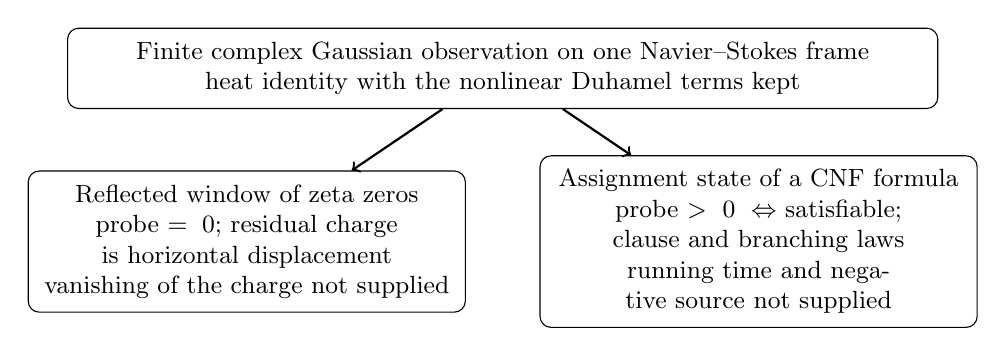
\begin{tikzpicture}[every node/.style={draw,rounded corners,
  align=center,inner sep=5pt,font=\small}]
\node[text width=10.7cm] (top) at (0,2.2)
  {Finite complex Gaussian observation on one Navier--Stokes frame\\
   heat identity with the nonlinear Duhamel terms kept};
\node[text width=5.2cm] (rh) at (-3.25,0)
  {Reflected window of zeta zeros\\
   probe $=0$; residual charge is horizontal displacement\\
   vanishing of the charge not supplied};
\node[text width=5.2cm] (sat) at (3.25,0)
  {Assignment state of a CNF formula\\
   probe $>0\Leftrightarrow$ satisfiable; clause and branching laws\\
   running time and negative source not supplied};
\draw[->,thick] (top) -- (rh);
\draw[->,thick] (top) -- (sat);
\end{tikzpicture}
\caption{One observation and one Navier--Stokes frame read on two
finite states.  The probe readouts differ, and each application keeps
its own hypotheses.}
\label{fig:triad-observation-span}
\end{figure}

\subsection{The limits of the common construction}

The difference between the two probe readouts is a mathematical
constraint.  If \(\varphi\) is satisfiable, no map
\(F:\mathbb R^{W}\to\mathbb R^{A_{n}}\), linear or not, can satisfy
\(L_{A_{n}}(F(v))=L_{W}(v)\) for every \(v\) and \(F(v_{W})=s_{\varphi}\):
it would send probe value \(0\) to a positive probe value.  This
excludes only maps of that kind; it says nothing about other transports
between the two settings.

The positivity test \eqref{eq:triad-sat-mass}, evaluated as written,
inspects all \(2^{n}\) assignments, and no polynomial-time evaluation
or precision bound for the Gaussian mass is proved.  Its terms can be as
small as \(e^{-\kappa(2^{n}-1)^{2}}\), so deciding positivity from a
fixed-point approximation of the mass with absolute error below the
smallest term would need a number of bits exponential in \(n\).  The P-versus-NP companion proves separately that a
polynomial-time SAT decider exists exactly when its tagged witness
selector is computable in polynomial time; admitting the resulting
transducer to a chosen family of current observables is a further
premise, and under that admission the accepted negative source has the
strength of \(L_{\mathrm{SAT}}\notin P\).  The Gaussian and residual
identities supply none of this.

Likewise, the zero-window premise must make the residual charge vanish,
and the Navier--Stokes closure must control high frequencies,
reconstruction and long times.  \Cref{thm:concrete-triad-gaussian-xi}
connects three objects through one kernel and one residual calculus
with exact identities; it gives no implication from the hypothesis of
one application to that of another, and it is not a single sufficient
condition for all three problems.
